\documentclass[9pt, apectratio=43,unicode]{beamer}
\usetheme{Moscow}

\usepackage[utf8]{inputenc}
\usepackage[T2A]{fontenc}
\usepackage[main=russian,english]{babel}

\usepackage{amsmath,amssymb}

\renewcommand{\thefootnote}{\fnsymbol{footnote}}
\hypersetup{pdfauthor={Paul Ostanin}}

%\usepackage{concmath}
%\usepackage{euler}

\usepackage{mathtools}

\graphicspath{ {images/} }

\title[Моделирование земной ионосферы]{Динамическое моделирование земной ионосферы}
\author[Останин П. А.]{Останин Павел Антонович \\ \vspace{1ex} Научный руководитель: Кулямин Дмитрий Вячеславович}
\date{}

\newcommand{\colorhref}[2]{\href{#1}{\textcolor{miptbase!30!black}{#2}}}

\begin{document}

\begin{frame}[plain]
\titlepage
\end{frame}

\def\L{\mathcal{L}}

\section{Введение}
\begin{frame}\frametitle{Постановка задачи}
Основные задачи:
\begin{itemize}
\item[•] Построение динамической трёхмерной модели Земной ионосферы;
\item[•] Согласование с уже разработанной моделью нейтральной термосферы ИВМ РАН.
\end{itemize}

Уравнение, описывающее эволюцию ионной концентрации: $$\dfrac{\partial n_i}{\partial t} = -div(n_i \vec{u}_\parallel)-div\left(n_i\dfrac{1}{B^2}[\vec{E}\times \vec{B}] \right)+$$ $$+div\left(D\left[\nabla_\parallel n_i +n_i\dfrac{1}{T_p}\nabla_\parallel T_p - \dfrac{n_i m_i}{2kT_p}\vec{g}_\parallel\right]\right)+[P-k_in_i]$$
\end{frame}


\subsection{Метод расщепления}
\begin{frame}\frametitle{Уравнение в сферических координатах в приближении тонкого сферического слоя}

$$\dfrac{\partial n_i}{\partial t} = DYZ(n_i)+DTr(n_i)+Tr(n_i)+[P-kn_i].$$

$$Tr(n_i) = \dfrac{1}{a\cos\varphi}\dfrac{\partial}{\partial\lambda}\left[n_i\dfrac{1}{B}(E_y\sin I + E_z\cos I)\right]+\dfrac{1}{a\cos\varphi}\dfrac{\partial}{\partial\varphi}\bigg[\bigg(u_z\sin I \cos I - u_y\cos^2 I -$$ $$- \dfrac{E_x}{B}\sin I\bigg)n_i\cos\varphi\bigg]+\dfrac{\partial}{\partial z}\left[\left(u_y\cos I \sin I -u_z\sin^2 I - \dfrac{E_x}{B}\cos I\right)n_i\right];$$

$$DYZ(n_i) = \dfrac{1}{a\cos\varphi}\dfrac{\partial}{\partial\varphi}\left(D\cos\varphi\left[\dfrac{1}{a}\dfrac{\partial n_i}{\partial\varphi} \cos^2 I -\dfrac{\partial n_i}{\partial z}\cos I\sin I\right]\right)+ \dfrac{\partial}{\partial z}\bigg(D\bigg[\dfrac{\partial n_i}{\partial z}\sin^2 I -$$ $$- \dfrac{1}{a}\dfrac{\partial n_i}{\partial\varphi}\cos I \sin I\bigg]\bigg);$$ 

$$DTr(n_i) = \dfrac{1}{a\cos\varphi}\dfrac{\partial}{\partial \varphi}\bigg[\bigg(\dfrac{1}{a}\dfrac{1}{T_p}\dfrac{\partial T_p}{\partial\varphi}\cos^2 I-\dfrac{1}{T_p}\dfrac{\partial T_p}{\partial z}\cos I \sin I - \dfrac{1}{H}\sin I \cos I\bigg)Dn_i\cos\varphi\bigg] +$$ $$+ \dfrac{\partial}{\partial z}\bigg[\bigg(-\dfrac{1}{a}\dfrac{1}{T_p}\dfrac{\partial T_p}{\partial \varphi}\cos I \sin I +\dfrac{1}{T_p}\dfrac{\partial T_p}{\partial z}\sin^2 I+\dfrac{1}{H}\sin^2I\bigg)Dn_i\bigg].$$
\end{frame}

\begin{frame}\frametitle{Метод расщепления}
\begin{itemize}
\item[•] На первом шаге расщепления решается уравнение для $z$-диффузии в проекции со смешанной производной;

$$\dfrac{\partial n}{\partial t} =P-kn+\dfrac{\partial}{\partial z}\biggl[D\sin^2 I\left(\dfrac{\partial n}{\partial z}+\left(\dfrac{1}{T_p}\dfrac{\partial T_p}{\partial z}+\dfrac{1}{H}\right)n\right)-$$ $$-\dfrac{1}{a}D\sin I\cos I\left(\dfrac{\partial n}{\partial\varphi}+\dfrac{1}{T_p}\dfrac{\partial T_p}{\partial\varphi}n\right)\biggr]$$ 
\item[•] На втором шаге добавляется диффузия по $y$. 
\item[•] На третьем шаге добавляется перенос.
\end{itemize}
\end{frame}


\section{Результаты численных экспериментов}
\subsection{Воспроизведение дневного вертикального профиля электронной концентрации}
\begin{frame}\frametitle{Воспроизведение дневного вертикального профиля электронной концентрации}
\begin{figure}[H]
\center{
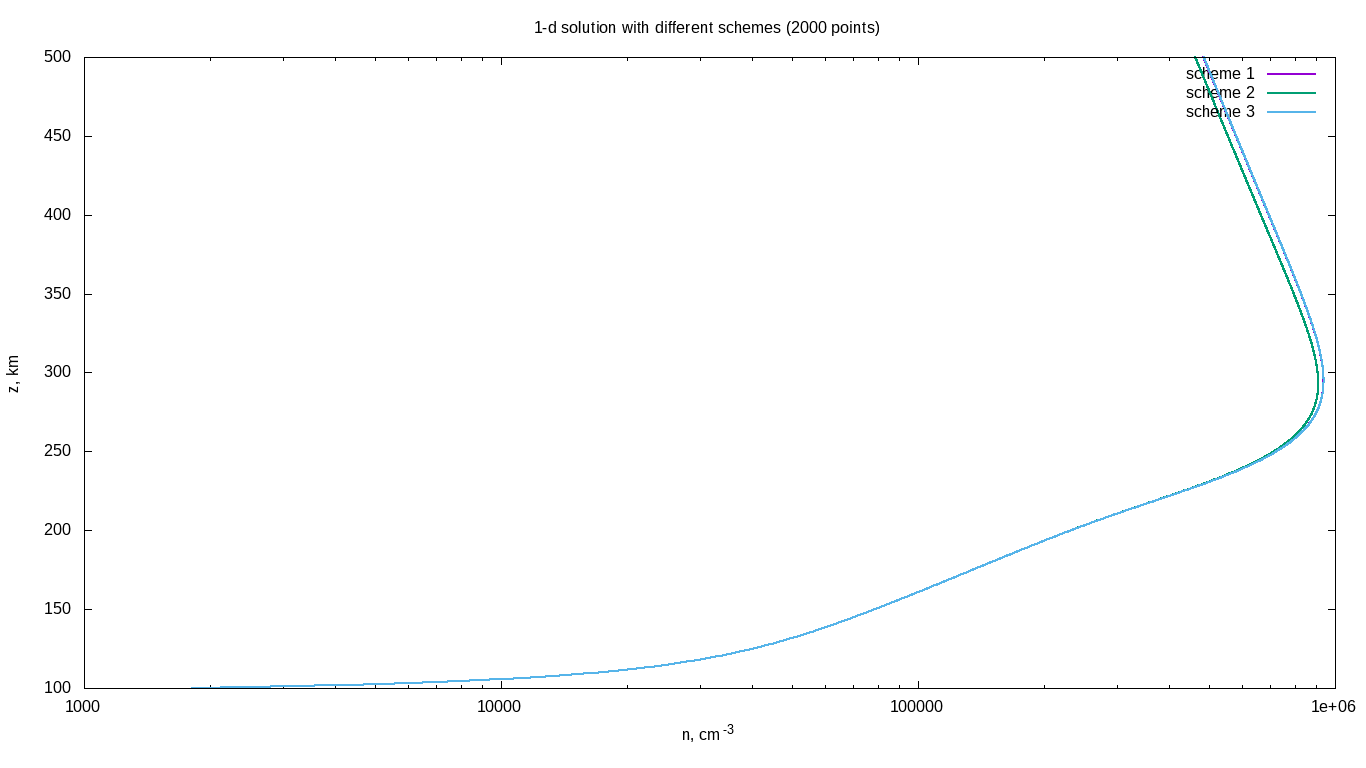
\includegraphics[scale=0.33]{1d_stationary_logscale_2000}}
\caption{Стационарные решения на $2000$ расчётных узлах.}
\end{figure}
\end{frame}


\subsection{Чувствительность к изменению внешних параметров}
\begin{frame}\frametitle{Чувствительность к изменению внешних параметров}

Варьирование входящих в уравнение температур показывает, что наибольшую чувствительность решение имеет к температуре нейтральных молекул.

\begin{figure}
\center{
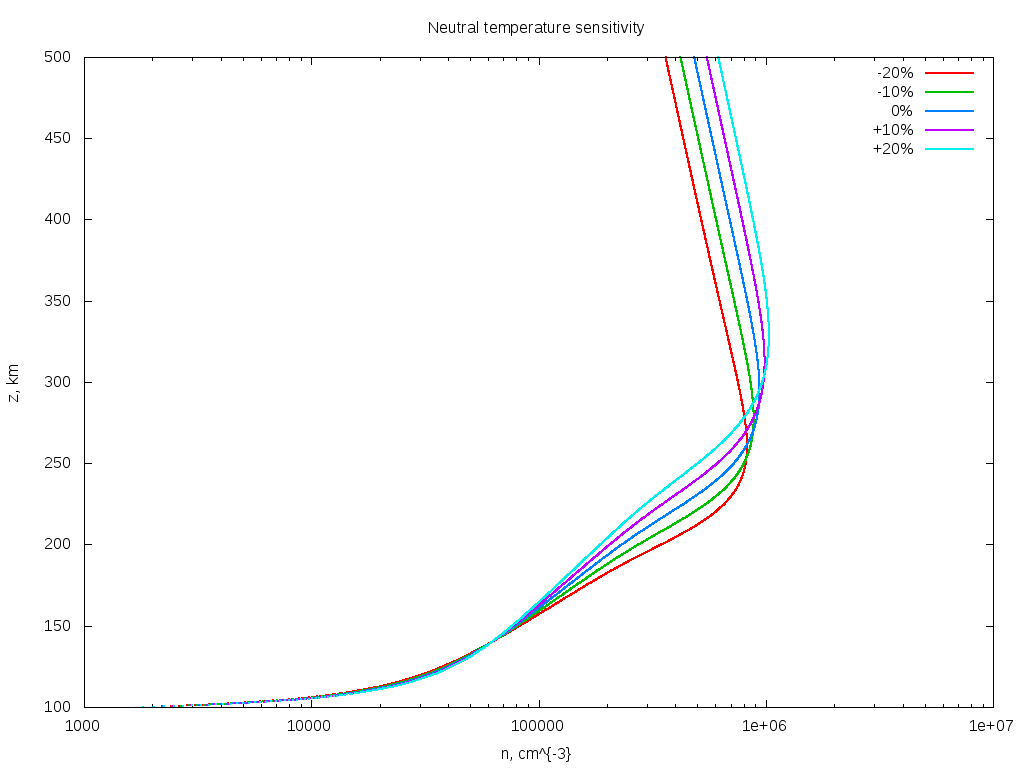
\includegraphics[scale=0.3]{Tn-sensitivity_log}}
\caption{Чувствительность к изменению температуры нейтральных молекул.}
\end{figure}
\end{frame}


\subsection{Моделирование суточного хода}
\begin{frame}\frametitle{Моделирование суточного хода}

Вычисляется стационарное решение одномерной задачи при дневном значении $P(z)$, затем итерации по времени продолжаются с меняющимся $P(z, t)$.

\begin{figure}[H]
\center{
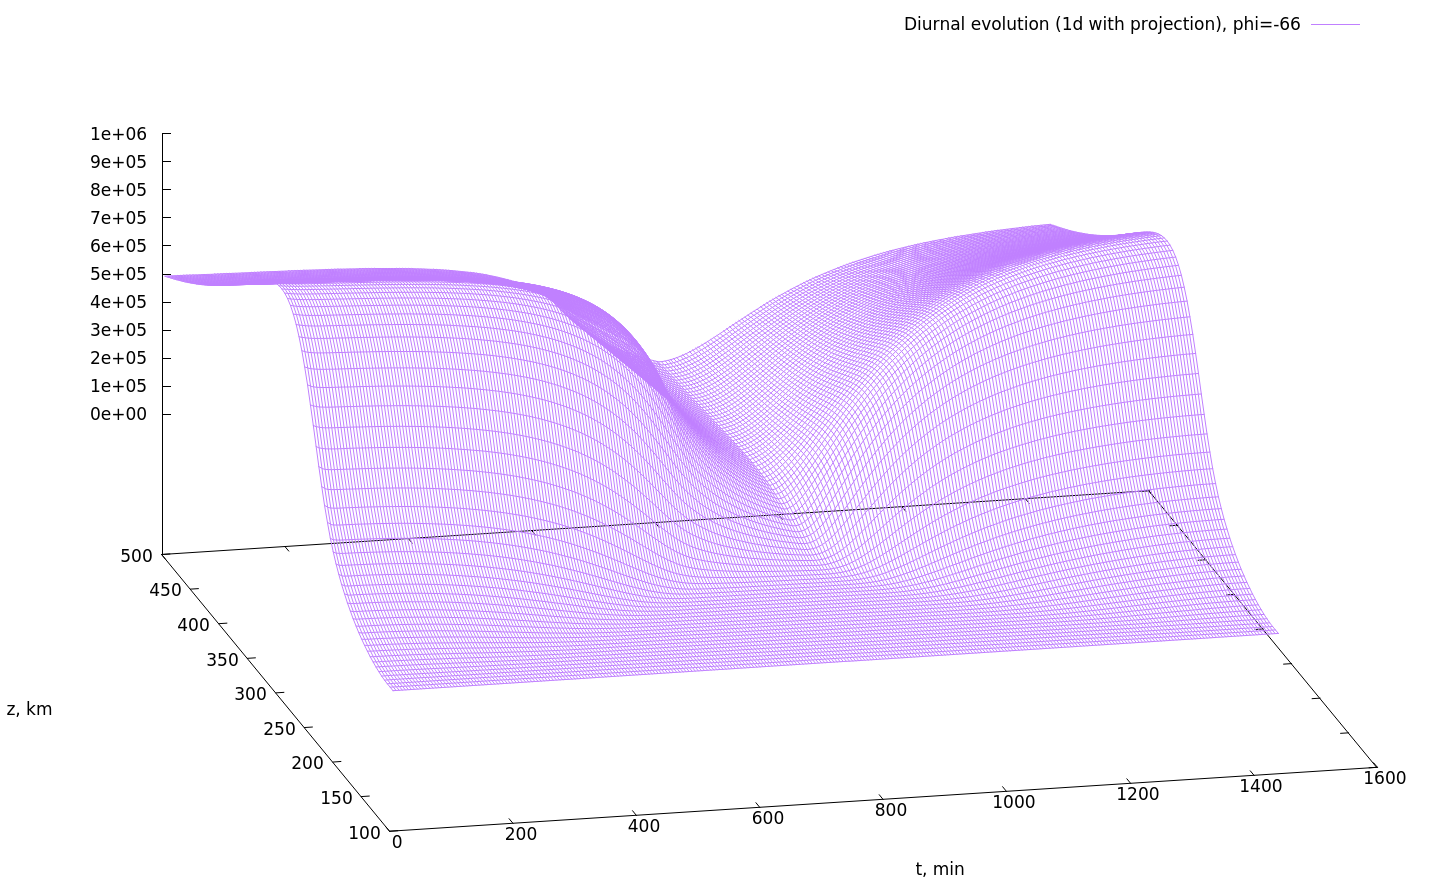
\includegraphics[scale=0.2]{diurnal_projection_-66}}
\caption{Суточный ход в одномерной модели с учётом проекции, $\varphi = -66^\circ$.}
\end{figure}

\end{frame}


\end{document}

